\documentclass[12pt,spanish]{article}
\usepackage[spanish]{babel}
\usepackage{graphicx}
\usepackage{svg}

\usepackage{multirow}
\usepackage{xfrac}
\usepackage{amsmath}
\usepackage{hyperref}
\usepackage{fixmath}
\usepackage{caption}
\usepackage{multicol}
\usepackage[skins,minted,breakable]{tcolorbox}
\usepackage{float}
\usepackage{array}
\graphicspath{ {./img/} {../../LaTeX/img/} {/home/csp98/latex/img/}}
\selectlanguage{spanish}
\usepackage[utf8]{inputenc}
\usepackage{graphicx}
\usepackage[a4paper,left=3cm,right=2cm,top=2.5cm,bottom=2.5cm]{geometry}
\newtheorem{ppio}{Principio }
\makeindex

\begin{document}
\begin{titlepage}

\newlength{\centeroffset}
\setlength{\centeroffset}{-0.5\oddsidemargin}
\addtolength{\centeroffset}{0.5\evensidemargin}
\thispagestyle{empty}

\noindent\hspace*{\centeroffset}
\begin{minipage}{\textwidth}

\centering
\includegraphics[width=0.9\textwidth]{logo_ugr.jpg}\\[1.4cm]

\textsc{ \Large Algorítmica\\[0.2cm]}
\textsc{GRADO EN INGENIERÍA INFORMÁTICA}\\[1cm]

{\Huge\bfseries Ejercicios ecuaciones de recurrencia\\}
\noindent\rule[-1ex]{\textwidth}{3pt}\\[3.5ex]
{\large\bfseries Método de expansión}
\end{minipage}

\vspace{1.5cm}
\noindent\hspace*{\centeroffset}
\begin{minipage}{\textwidth}
\centering

\textbf{Autor}\\ {Carlos Sánchez Páez}\\[2.5ex]
\includegraphics[width=0.3\textwidth]{etsiit_logo.png}\\[0.1cm]
\vspace{1.5cm}
\includegraphics[width=0.5\textwidth]{decsai.jpg}\\[0.1cm]
\vspace{1cm}
\textsc{Escuela Técnica Superior de Ingenierías Informática y de Telecomunicación}\\
\vspace{1cm}
\textsc{Curso 2017-2018}
\end{minipage}
\end{titlepage}
\tableofcontents
\listoffigures
\thispagestyle{empty}
\newpage
\setcounter{page}{1}

\section{Enunciado}

\textbf{Ejercicio}. Resuelva las siguientes ecuaciones de recurrencia mediante el método de \textit{expansión}.

\begin{equation}
T(n)=2T(\frac{n}{2})+1 \quad \text{con T(1)=1}
\end{equation}
\begin{equation}
T(n)=2T(\frac{n}{2})+n \quad \text{con T(1)=1}
\end{equation}

\section{Resolución}
El método de expansión consiste en ir resolviendo la ecuación de la forma $T(n-i)$ hasta que llegue un punto en el que podamos obtener un patrón de resolución del que hallaremos una ecuación.
En ese momento, aplicaremos la ecuación al caso base y acotaremos mediante la notación \textbf{O(n)}.
\subsection{Ecuación 1}
\[T(n)=2T(\frac{n}{2})+1 \quad \text{con T(1)=1}\]
Comenzamos desarrollando la ecuación para $i=1$
\[T(n-1)=2 \cdot \left[2T(\frac{n-1}{2})+1\right]+1 = 4T(\frac{n-1}{2})+3\]
Seguimos ahora con $i=2$
\[T(n-2)=4 \cdot \left[2T(\frac{n-2}{2})+1\right]+3 = 8T(\frac{n-2}{2}) + 7 \]
Intuimos el patrón que sigue la recurrencia:
\[T(n)=
\begin{cases}
	1 & \quad \text{si } n = 1  \\
	2^{i+1} \cdot T(\frac{n-i}{2}) + 2^{i+1}-1 & \quad \text{en otro caso}
\end{cases}
\]
Lo comprobamos para $i=3$
\begin{enumerate}
\item Por expansión
\[ T(n-3)=8 \cdot \left[2T(\frac{n-3}{2})+1\right]+7=16T(\frac{n-3}{2})+15\]
\item Mediante la ecuación del patrón
\[ T(n-3)=2^{3+1} \cdot T(\frac{n-3}{2}) + 2^{3+1} - 1 = 16T(\frac{n-3}{2})+15 \]
\end{enumerate}
Por tanto, nuestro patrón era acertado. Ahora, aplicamos al \textit{caso base} ($i=n-2$)

\begin{equation}
\begin{split}
&T\left[n-(n-2)\right]=T(2)=2^{(n-2)+1} \cdot T(\frac{n-(n-2)}{2})+2^{(n-2)+1}-1= \\
&= 2^{n-1} \cdot T(1) + 2^{n-1}-1 = 2^{n-1} + 2^{n-1}-1 = 2^{n} -1 
\end{split}
\end{equation}

\begin{center}
Por tanto, concluimos que $T(n)$ es del orden de $O(2^{n})$ en la notación \textbf{O}.
\end{center}

\subsection{Ecuación 2}
\[T(n)=2T(\frac{n}{2})+n \quad \text{con T(1)=1}\]
Igual que en el apartado anterior, comenzamos desarrollando para $i=1$
\[T(n-1)=2 \cdot \left[2T(\frac{n-1}{2})+n\right]+n=4T(\frac{n-1}{n})+3n \]
Procedemos para $i=2$
\[T(n-2)=4 \cdot \left[2T(\frac{n-2}{2}+n\right]+3n=8T(\frac{n-2}{2})+7n \]
Vemos que el patrón de la ecuación es probablemente el siguiente: 
\[T(n)=
\begin{cases}
	1 & \quad \text{si } n = 1  \\
	2^{i+1} \cdot T(\frac{n-i}{2}) + (2^{i+1}-1)n & \quad \text{en otro caso}
\end{cases}
\]
Comprobamos para $i=3$
\begin{enumerate}
\item Por expansión
\[ T(n-3)=8 \cdot \left[2T(\frac{n-3}{2})+n\right]+7=16T(\frac{n-3}{2})+15n\]
\item Mediante la ecuación del patrón
\[ T(n-3)=2^{3+1} \cdot T(\frac{n-3}{2}) + (2^{3+1} - 1)n = 16T(\frac{n-3}{2})+15n \]
\end{enumerate}
Por tanto, nuestro patrón es correcto.
Aplicamos al \textit{caso base} ($i=n-2$):
\begin{equation}
\begin{split}
&T\left[n-(n-2)\right]=T(2)=2^{(n-2)+1} \cdot T(\frac{n-(n-2)}{2})+(2^{(n-2)+1}-1)n= \\
&= 2^{n-1} \cdot T(1) + (2^{n-1}-1)n = 2^{n-1} + (2^{n-1}-1)n = (2^{n-1}-1)n +2^{n-1} 
\end{split}
\end{equation}
\begin{center}
Por tanto, podemos concluir que la ecuación $T(n)$ es del orden de $O(n \cdot
2^{n})$ en notación \textbf{O}.
\end{center}
\section{Gráficas}
\subsection{Ejercicio 1}
\begin{figure}[H]
\centering
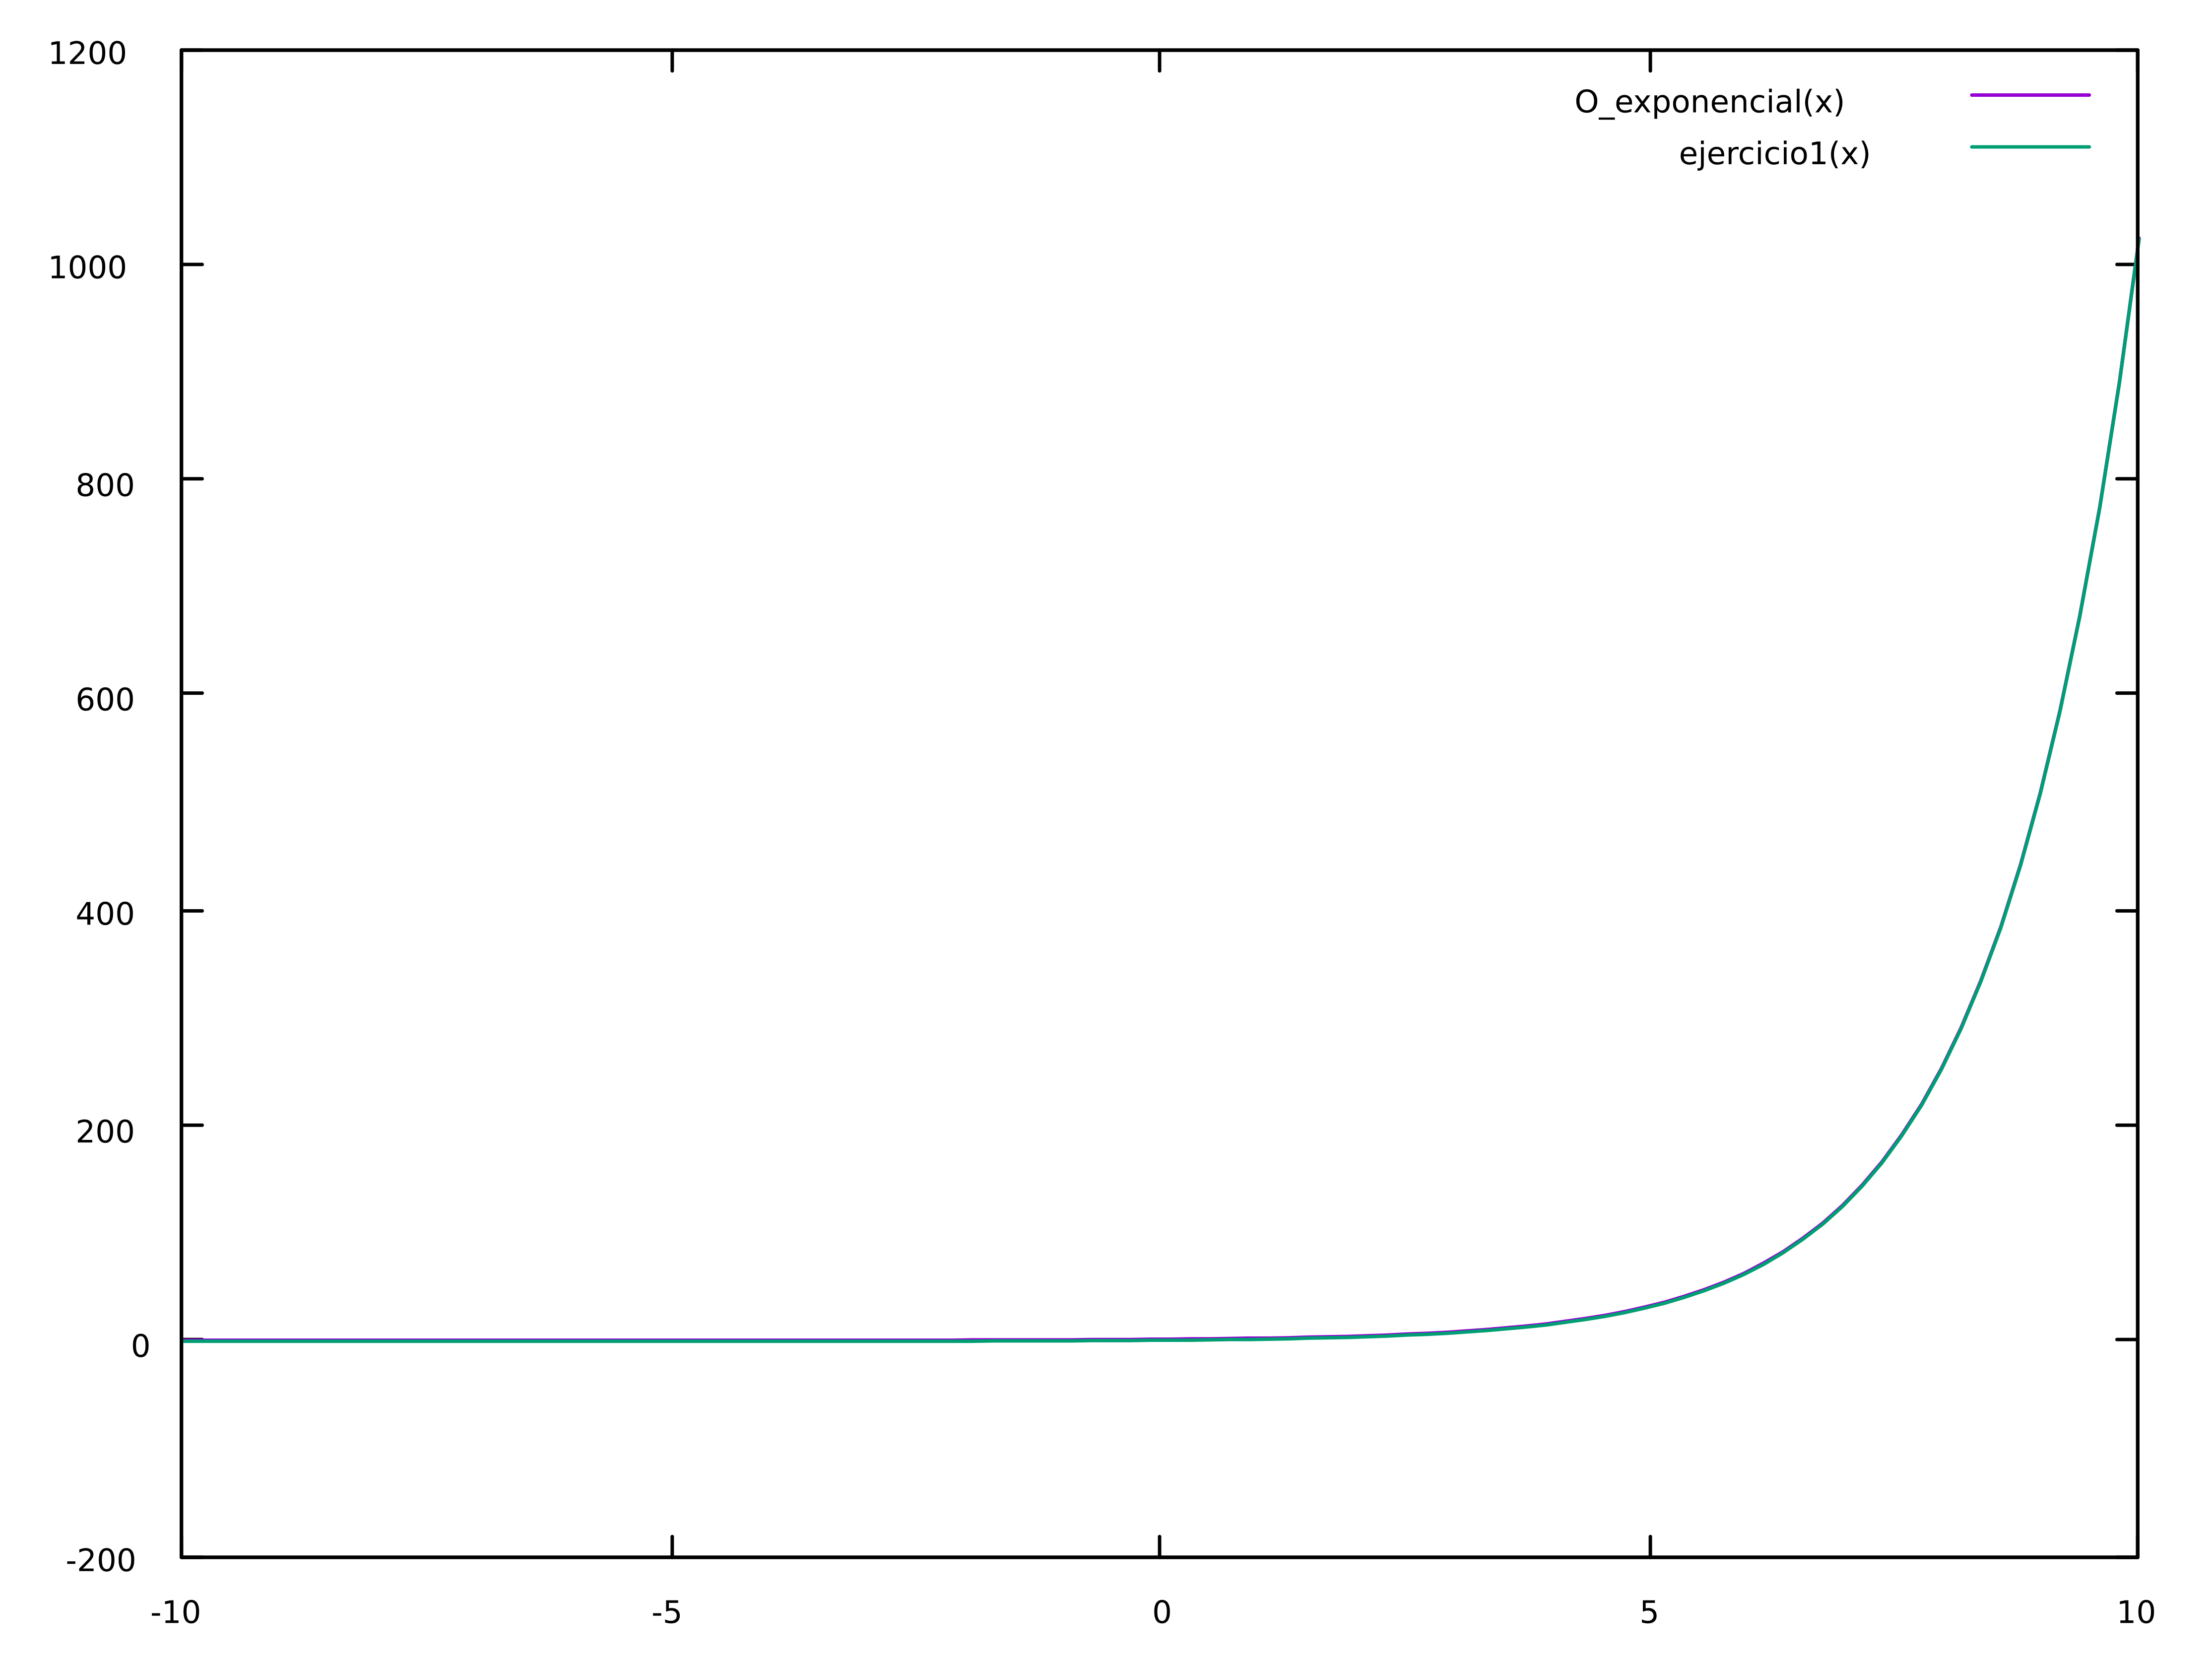
\includegraphics[scale=0.55]{ej1.png}
\caption{Representación de $2^{n}$ y $2^{n}-1$}
\end{figure}

\begin{figure}[H]
\centering
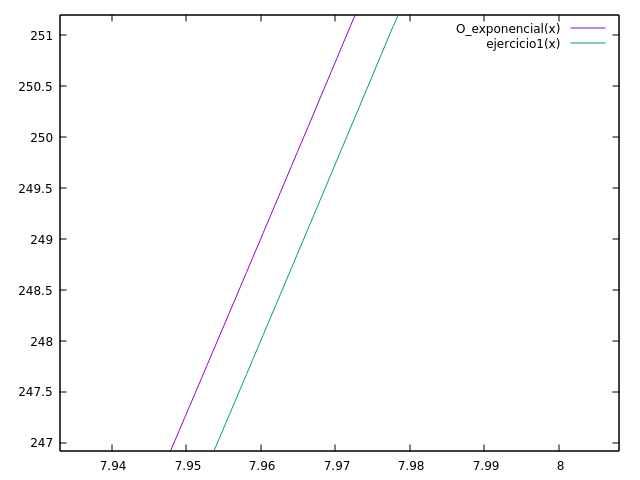
\includegraphics[scale=0.75]{ej1_zoom.png}
\caption{Ampliación de $2^{n}$ y $2^{n}-1$}
\end{figure}

\subsection{Ejercicio 2}

\begin{figure}[H]
\centering
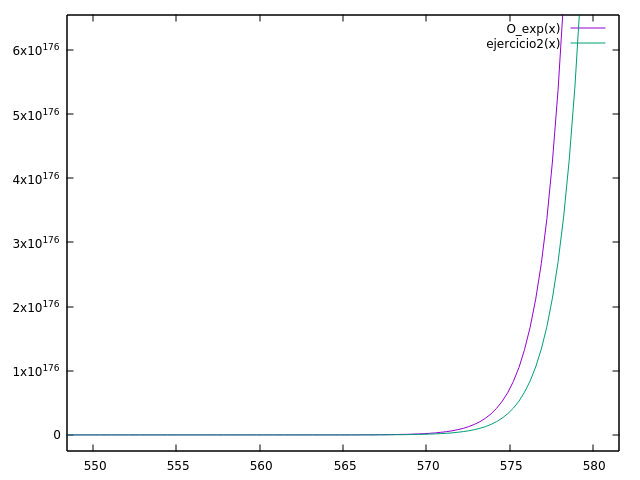
\includegraphics[scale=0.75]{ej2.png}
\caption{Representación de $n \cdot 2^{n}$ y $(2^{n-1}-1)n +2^{n-1}$}
\end{figure}

\begin{center}
Como podemos ver, en ambos casos las funciones son acotadas por su \textbf{O(f(n))} correspondiente.
\end{center}
\end{document}